%% 
%% Master Thesis
%% Autor: Martin Wichmann
%% 
%% Todo:
%% - Danksagung
%% - Cite auf mein GitHub ändern oder so?!
%% - Portabilität PC VM auf embedded Hypervisor
%% - Relevanz für Testen und Entwicklungsprozess


\documentclass[
  a4paper,					    % a4paper (sic!)
  %BCOR10mm,				    % Korrektur des innneren Randes bei Bindung (Bindungskorrektur)
  %DIV12,					    % je groesser die Zahl, desto kleiner der Rand
  %11pt,        			    % Schriftgroesse
  %oneside,
  twoside,
  %openright,   				% doppelseitig und jedes Kapitel faengt auf der rechten Seite an
  %pagesize,					% schreibt die Seitengroesseninformationen in die PDF Datei
  DIV=calc,     				% KOMA-Script soll den optimalen Satzspiegel berechnen
  %DIVclassic, 					% mittelalterlicher Buchseitenkanon
  %headsepline,					% Trennlinie
  %footsepline,					% Trennlinie
  %headtopline,					% Trennlinie
  %footbotline,					% Trennlinie
  %noonelinecaption,			% setzt die Bildueberschrift unabhaengig von der Laenge immer linksbuendig
  %liststotoc,
  %idxtotoc,
  bibliography=totoc,
  %bibtotocnumbered, liststotocnumbered,
  %liststotoc, idxtotoc, bibtotoc,
  %tablecaptionbelow,
  %tablecaptionabove,	        % Tabellenbeschriftung unter oder oben
  %abstracton,  				% Überschrift der Zusammenfassung aktivieren
  %chapterprefix,				% "Kapitel xx" vor jeder Kapitelueberschrift
  %cleardoublestandard,
  %cleardoubleplain,
  cleardoublepage=empty,
  %smallheadings,
  %normalheadings,
  %makeidx,
  ngerman,     					% allen Paketen die Hauptsprache mitteilen
  %draft       					% draft version  
  final       					% final version
]{scrbook}	
%%%%%%%%%%%%%%% Grundlegendes %%%%%%%%%%%%%%%
\usepackage[utf8]{inputenc}
\usepackage[T1]{fontenc}
\usepackage[english,ngerman]{babel} 	% Unterstuezung fuer englisch und deutsch
\usepackage{setspace}			% erlaubt 1 1/2 fachen Zeilenabstand
%%%%%%%%%%%%%%% Tabellen %%%%%%%%%%%%%%%
%\usepackage{array}
%\usepackage{tabularx}
\usepackage{booktabs}			% \toprule, \midrule und \bottomrule in Tabellen
\usepackage{multirow}
%%%%%%%%%%%%%%% Mathe %%%%%%%%%%%%%%%
%\usepackage{amsmath, amsthm, amscd, amssymb, amsfonts}
%\usepackage{ziffer}
%\usepackage{icomma}
%%%%%%%%%%%%%%% Typografie %%%%%%%%%%%%%%%
%\usepackage{mparhack}			% workaround for a LaTeX bug in marginpars
\usepackage{ellipsis}			% fix uneven spacing around ellipses in LaTeX text mode.
\usepackage{microtype} 			% optischer Randausgleich (font expansion and character protrusion)
%%%%%%%%%%%%%%% Schriften %%%%%%%%%%%%%%%
\usepackage{lmodern}
%\usepackage{textcomp} 			% Sonderzeichen
%\usepackage{mathcomp}
%\usepackage{chemsym}
%%%%%%%%%%%%%%% Sonstiges %%%%%%%%%%%%%%%
%\usepackage{url}
\usepackage{scrhack}            % KOMA Paket um zussammenarbeit mit anderen Paket (listings) zu verbessern
\usepackage{listings}			% Code-Abschnitt mit Syntax-Highlighting
\lstset{
%language=C,
breaklines=true,
breakatwhitespace=true
basicstyle=\footnotesize,
numbers=left,
numberstyle=\footnotesize,
stepnumber=2,
numbersep=5pt,
extendedchars=true,
inputencoding=utf8,
breakindent=30pt,
escapeinside={\%(}{\%)},
%xleftmargin=20pt				% Einrückung der listings
}
%\usepackage{color} 			% Farben
%%%%%%%%%%%%%%% Grafiken %%%%%%%%%%%%%%%
\usepackage[pdftex]{graphicx}	% das pdftex soll das Handling von Bildern verbessern
\graphicspath{{images/}}		% Bilder im Verzeichnis images suchen
\usepackage{wrapfig}
%\usepackage[hang]{subfigure}	% Subabbildungen
%\usepackage{tikz}				% zum Zeichnen (Frontend zu PGF)
\usepackage{pgfgantt}           % pgf verwenden um Gantt Diagramme zu erstellen
%\usepackage{rotating} 			% fuer gedrehte Tabellen und Bilder
%\usepackage{pdfpages}
\usepackage[
  pdftex,
  bookmarks, bookmarksopen, bookmarksopenlevel=1, bookmarksnumbered=true,
  pdfpagemode={UseNone},		% UseNone, FullScreen, UseThumbs, UseOutlines, (UseOC, UseAttachments)
  pdfpagelayout={TwoPageRight},	% SinglePage, OneColumn, TwoColumnLeft, TwoColumnRight, TwoPageLeft, TwoPageRight
  plainpages=false, 
  pdfkeywords={},
  pdfsubject={},
  pdftitle={Master-Arbeit},
  pdfauthor={Martin Wichmann}
]{hyperref}
%%%%%%%%%%%%%%% Zitieren und Index %%%%%%%%%%%%%%%
% Ich habe im Internet gelesen, dass cite nach hyperref stehen soll?!
\usepackage[numbers]{natbib}
% Index:
%\usepackage{makeidx}					% Paket für die Indexerstellung
%\makeindex
% Glossar:
%\usepackage[style=super, header=none, border=none, number=none, cols=2, toc=true]{glossary}
%\usepackage[style=altlist, number=none]{glossary}
%\makeglossary
% Benutzung des Glossars: \glossary{name={Schnauze}, description={Fachausdruck für die Hundenase.},}
%                         \glossary{name={Knochen}, description={Lieblingsspeise eines jeden Hundes.},}
%%%%%%%%%%%%%%%%%%%%%%%%%%%%%%%%%%%%%%%%%%%%%%%%%%%%

%%%%%%%%%%%%%%%%%%%%%%%% Eigene Definitionen %%%%%%%%%%%%%%%%%%%%%%%%%%%%%%

%%% Bei Verwendung von BibTex: %%%%%%%%%%%%%%%%%%%%
\addto{\captionsngerman}{\renewcommand*{\bibname}{Quellenverzeichnis}}
% sonst
%\renewcommand{\bibname}{Quellenverzeichnis}

%%% Trennungen %%%%%%%%%%%%%%%%%%%%%%%%%%%%%%%%%%%%%%%%%%%
\hyphenation{}

%%% 1 1/2 fachen Zeilenabstand wählen %%%%%%%%%%%%%%%%%%%%
\onehalfspacing
\typearea[current]{calc}				% Neuberechnung des Satzspiegels

%%%%%%%%%%%%%%%%%%%%%%%%%%%% Begin document %%%%%%%%%%%%%%%%%%%%%%%%%%%%%%%
\begin{document}
\selectlanguage{ngerman}
\frontmatter

%%%%%%%%%%%%%%%%%%%%%%%%%%%%%%%%% Titel %%%%%%%%%%%%%%%%%%%%%%%%%%%%%%%%%%
\titlehead{\center{\large \textsc{Ostfalia Hochschule für angewandte Wissenschaften}}}
\subject{Master-Arbeit}
\title{Virtualisierung von Autosar Softwarekomponenten für die Erprobung}
\author{Martin Wichmann\\Matrikel 701\,277\,37}
\date{Eingereicht am TODO}
\publishers{Prüfer: 

  Prof. Dr.-Ing. Gert Bikker

  Prof. Dr.-Ing. Jürgen Kreyßig

  }

%\uppertitleback{%
%  Beteiligte Institutionen:\\
%  \parbox{0.5\textwidth}{%
%  \centering \includegraphics[width=3.5cm]{logofh} \\
%  Fakultät Informatik \\ Ostfalia Hochschule für angewandte Wissenschaften } \hfill
%}


% TODO: github cite in footnote ändern?!
\lowertitleback{Diese Arbeit wurde mit Hilfe von Freier Software erstellt: \\
Gesetzt mit Hilfe von {\KOMAScript} und {\LaTeX}. LibreOffice für die \\ Textverarbeitung und gedit als Editor. Xubuntu als offenes Betriebssystem. \\ \\ Diese Arbeit ist freigegeben unter der Creative Commons CC-BY-SA Lizenz\cite{CCBYSA} und ist im Internet erreichbar\cite{github}.
}
% TODO: evtl. qoute ändern ;-)
\dedication{Do or do not...there is no try!\\ \vspace{1cm}
\textit{Yoda}
}

\begin{singlespace}
\maketitle

%%%%%%%%%%%%%%%% Abstract %%%%%%%%%%%%%%%%%%%%%%%


\section*{Zusammenfassung}
\pdfbookmark[1]{Zusammenfassung}{Zussammenfassung}
TODO
\vfill

\foreignlanguage{english}{
\section*{Abstract}
TODO
\vfill
}


\thispagestyle{empty}

%%%%%%%%%%%%%%%%%%%%%%%%%%%%%% Verzeichnisse %%%%%%%%%%%%%%%%%%%%%%%%%%%%%%

\tableofcontents               	% Inhaltsverzeichnis
%\listoffigures               		% Abbildungsverzeichnis
%\listoftables             			% Tabellenverzeichnis
%\lstlistoflistings          		% Listenverzeichnis
%\listoflistings					% Quellcodeverzeichis
%\printglossary               		% Formelverzeichnis
\end{singlespace}


%%%%%%%%%%%%%%%%%%%%%%%%%%%%%% Zeilenabstand %%%%%%%%%%%%%%%%%%%%%%%%%%%%%%
% Das Setzen eines anderen Abstandes mitten im Dokument kann zu Fehlern führen (vgl. scrguide S. 30)
%\doublespacing
%\onehalfspacing
%\typearea[current]{last}					% stammt aus scrguide S. 30
%\typearea[current]{calc}					% Neuberechnung des Satzspiegels









%%%%%%%%%%%%%%%%%%%%%%%%%%%%%%% Einleitung %%%%%%%%%%%%%%%%%%%%%%%%%%%%%%%%%%
\mainmatter
\chapter{Einleitung}
\label{sec:Einleitung}
% TODO

Diese Master-Arbeit betrachtet die Möglichkeiten der Virtualisierung im Embedded Bereich anhand eines Fallbeispiels. Dieses Fallbeispiel wird im nächsten Kapitel vorgestellt. Anschließend werden die theoretischen Grundlagen erläutert und diskutiert. Die praktische Umsetzung des Fallbeispiels wird danach erläutert. Zum Schluss werden einige Aspekte werden einige Aspekte dieser Arbeit analysiert und die Relevanz für die Wirtschaft betrachtet.





%%%%%%%%%%%%%%%%%%%%%%%%%%%%%%% Vorstellung Fallbeispiel %%%%%%%%%%%%%%%%%%%%%%%%%%%%%%%%%%
% Gesamtes Modell darstellen
\chapter{Motivation und Planung}
\label{sec:MotivationPlanung}
% TODO
Das in dieser Master-Arbeit betrachtete Praxis-Beispiel ist eine Scheinwerfer-Steuerung inklusive User-Interface. Dies ist bewusst als minimal Beispiel konzipiert um den Fokus auf die Virtualisierung zu legen.

\begin{figure}[ht]
\centering
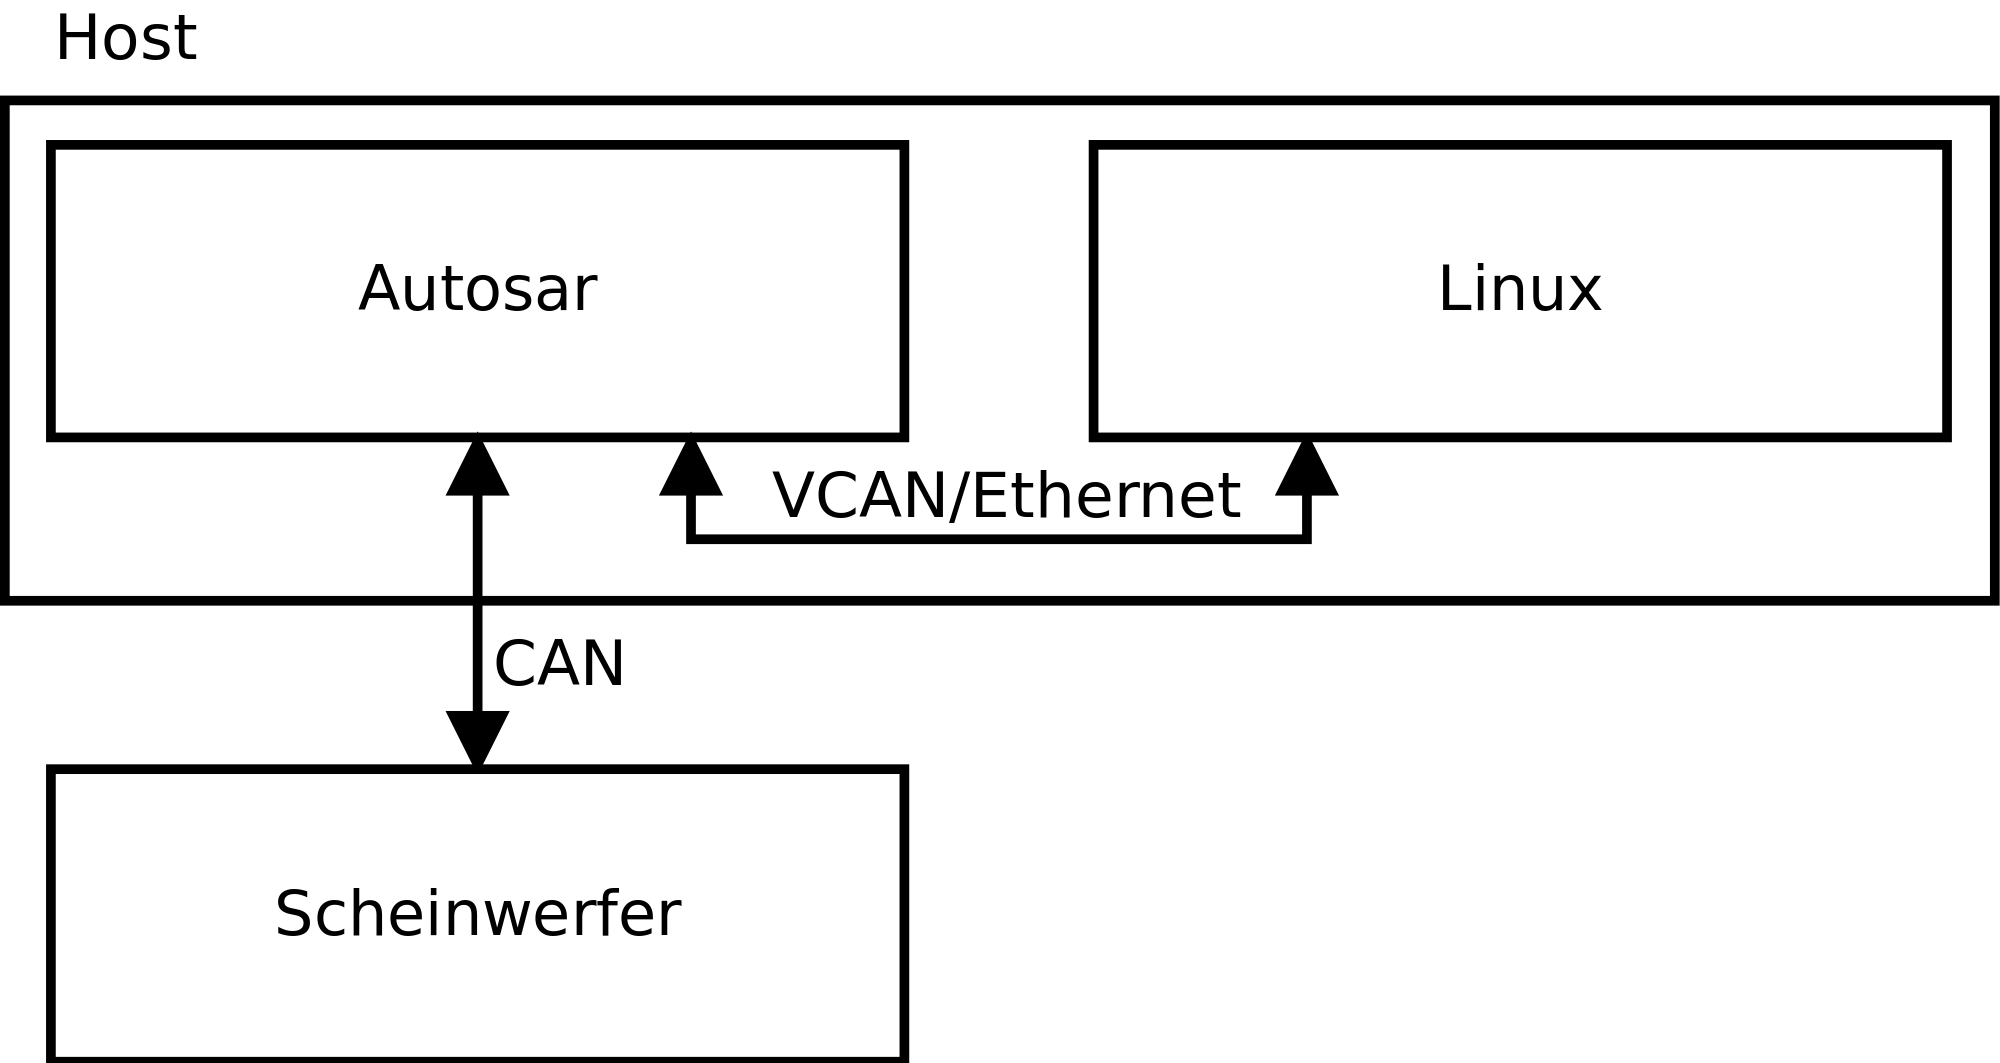
\includegraphics[width=0.8\textwidth]{overview.png}
\caption{Architektur}
\label{fig:arch}
\end{figure}

Die geplante Architektur der Scheinwerfer-Steuerung ist in Abbildung \ref{fig:arch} zu sehen. Dabei sind zwei getrennte Hardware Elemente zu sehen. Zum einen das Scheinwerfer-Steuergerät und zum anderen das in dieser Arbeit betrachtete System. Das Steuergerät übernimmt die direkte Steuerung der Scheinwerfer und ist per CAN-Bus mit dem anderen System verbunden.  Dieses beherbergt ein virtuelles Autosar und Linux auf einem Windows Host.

Aus dieser Architektur-Beschreibung lassen sich vier Kern-Bereiche dieser Master-Arbeit ableiten:

\begin{itemize}
    \item Virtualisierung von Autosar und Linux
    \item Kommunikation zwischen Linux und Autosar
    \item Kommunikation zwischen Autosar und Scheinwerfer
    \item Zugriff auf Hardware inklusive Betrachtung von Netzwerkmanagement
\end{itemize}

Hierbei ist zu beachten, dass das aktivieren des Netzwerkmanagements erst möglich ist, sobald eine Kommunikation zwischen Autosar und der Hardware möglich ist.

% TODO: Projektplanung
Da der Zeitaufwand für die einzelnen Phasen nur sehr schwer einzuschätzen ist, wird für jede Phase des Projektes ein Monat Arbeit vorgesehen. Dazu kommen noch ein Monat Evaluation und Sicherheitsbetrachtung des Systems und zum Schluss ein Monat Fertigstellen der schriftlichen Arbeit. Die Zeitplanung ist in einem Gantt-Diagramm in Abbildung \ref{fig:gantt} zu sehen. Jede Phase enthält die Vorbereitung, Umsetzung und Dokmentation des entsprechenden Bereichs.


\begin{figure}[ht]
\centering

\begin{ganttchart}{12}
\gantttitle{2012}{8} 
\gantttitle{2013}{4} \\
\gantttitlelist{9,10,11,12,1,2}{2} \\
\ganttbar{Virtualisierung}{1}{2} \\
\ganttbar{Kommunikation Linux/Autosar}{3}{4} \\
\ganttbar{Kommunikation Autosar/Scheinwerfer}{5}{6} \\
\ganttbar{Zugriff auf Hardware}{7}{8} \\
\ganttbar{Evaluation}{9}{10} \\
\ganttbar{Fertigstellen der Arbeit}{11}{12} 
\end{ganttchart}

\caption{Zeitplanung Master-Arbeit}
\label{fig:gantt}
\end{figure}




%%%%%%%%%%%%%%%%%%%%%%%%%%%%%%% Grundlagen %%%%%%%%%%%%%%%%%%%%%%%%%%%%%%%%%%
\chapter{Grundlagen}
\label{sec:Grundlagen}
Dieses Kapitel enthält Grundlagen zu den Themen Autosar und Virtualisierung.
% TODO


%%%%%%%%%%%%%%%%%%%%%%%%%%%%%%% Virtualisierung %%%%%%%%%%%%%%%%%%%%%%%%%%%%%%%%%%
% Allgemeine Virtualisierung
% Class 1 und 2
\section{Virtualisierung}
\label{sec:Virtualisierung}
Der Begriff Virtualisierung bezeichnet eine Reihe von Techniken die verwendet werden um die Ressourcen eines Rechner-Systems zu verwalten. Hierdurch kann eine reales System als mehrere logische betrachtet und genutzt werden. Dabei können verschiedene Ziele verfolgt werden.

Aus dem Desktop-Bereich ist die System-Virtualisierung bekannt wie sie zum Beispiel mittels VirtualBox\footnote{VirtualBox zu finden unter \url{www.virtualbox.org}} umgesetzt ist. Hierbei werden die Ressourcen des bestehenden Systems durch einen Hypervisor verwaltet und den virtuellen Instanzen zugeordnet. Diese Art wird vor allem verwendet um zum Beispiel unter Windows Zugriff auf ein Linux zu haben um spezielle Software auszuführen.

Im Gegensatz dazu wird im Server-Bereich der Fokus auf andere Bereiche gelegt. Die hier verfolgten Ziele sind vor allem eine einfache Wartbarkeit, Ausfallsicherheit und Ressourcenschonung. Mittels virtueller Server können Ausfallzeiten minimiert werden, indem bei einem Ausfall einfach eine andere virtuelle Instanz des Servers gestartet wird und dessen Arbeit übernimmt. 

Virtualisierung kann mittels einer Reihe von Techniken erfolgen. Hier wird zum Beispiel Unterschieden ob die Hardware direkt zum Gast-System weitergegeben wird, oder aber eine eigene virtuelle Hardware emuliert wird. Außerdem könnte ein Gast-System Teile des Hosts, zum Beispiel dessen Kernel, mit verwenden. Allgemein werden die Hypervisor jedoch nach folgenden zwei Klassen unterschieden\cite[Seite 22 ff.]{hypervisor}:

\paragraph{Type 1 (bare host)} Hierbei handelt es sich um native Hypervisor die direkt auf der Hardware laufen. Diese bauen auf kein Betriebssystem auf und verwalten selbstständig die Ressourcen und Gast-Systeme. Aus diesem Grund sind sie vor allem Interessant für eingebettete Systeme. Type 1 Hypervisor werden genauer im nächsten Kapitel betrachtet.

\paragraph{Type 2 (extended host)} Ein Type 2 Hypervisor ist nur auf einem vollständigen Betriebssystem lauffähig. Damit ist der Hypervisor eine logische Schicht zwischen dem Host- und Gast-Betriebssystem und kann von den Vorteilen eines Betriebssystems profitieren. Hieraus ergibt sich das ein Type 2 Hypervisor meißt kleiner und schneller ist.





%%%%%%%%%%%%%%%%%%%%%%%%%%%%%%% Embedded Virtualisierung %%%%%%%%%%%%%%%%%%%%%%%%%%%%%%%%%%
% Gründe für Embedded Virtualisierung
\section{Virtualisierung bei eingebetteten Systemen}
\label{sec:EVirtualisierung}
Virtualisierung im Bereich der eingebetteten Systeme hat in den letzten Jahren immer mehr an Bedeutung gewonnen. Da Mikrocontroller und SOCs\footnote{System-on-a-Chip, dt. Ein-Chip-System} immer Leistungsfähiger werden ist es sinnvoll diese Leistung auch auszunutzen. Gerade im Automobil-Bereich, in dem die Anzahl der Steuergeräte zum Teil auf mittlerweile über 50 gestiegen ist, kann es die Kosten erheblich reduzieren wenn stattdessen einige dieser System virtualisiert werden können.

Hypervisor im embedded Bereich müssen bestimmte Erforderungen erfüllen die viele Hypervisor nicht betrachten. Zu diesen Anforderungen gehört zum Beispiel ein geringer Engerie-Verbrauch und Effiziente Speicher Nutzung. Ein weiterer wichtiger Punkt ist die Echtzeitfähigkeit. Diese ist vor allem kritisch, da meißt eine zwei-stufige Scheduler-Architektur entsteht, einmal der Scheduler des Hypervisors und einmal der Scheduler des Gast-Systems. Eine Echtzeit-Analyse ist in diesem Fall relativ anspruchsvoll.

Um nur ein einfaches Beispiel zu nennen, könnte ein System mit 4 Sub-Systemen betrachtet werden. Diese Sub-Systeme könnten alle in ein einziges System mit einer 4-Kern CPU vereint werden und genauso wie vorher verwendet werden. Je nach benötigter Leistung könnte das Resultierende System durchaus noch verkleinert und damit kostengünstiger gestaltet werden.


\subsection{Hypervisor Beispiel}
% Beispiele genauer betrachten: PikeOS, COQOS
% http://www.opensynergy.com/Products/COQOS
% http://www.windriver.com/products/hypervisor/
% http://www.ok-labs.com/products/okl4-microvisor
% http://www.lynuxworks.com/embedded-linux/embedded-linux-virtualization.php
% http://www.sysgo.com/products/pikeos-rtos-and-virtualization-concept/embedded-virtualization/
Im Bereich der Embedded Hypervisor gibt es eine Reihe verbreiteter Produkte. Dazu gehören zum Beispiel PikeOS\footnote{\url{http://www.sysgo.com/products/pikeos-rtos-and-virtualization-concept/embedded-virtualization/}}, OKL4\footnote{\url{http://www.ok-labs.com/products/okl4-microvisor}}, Integrity Multivisor\footnote{\url{http://www.ghs.com/products/rtos/integrity_virtualization.html}} und COQOS\footnote{\url{http://www.opensynergy.com/Products/COQOS}}.





\subsection{Vorteile}
% TODO Vorteile
Der Einsatz von Virtualisierung hat eine Reihe von Vorteilen\cite{wiki:emb_hyp}.

\paragraph{Betriebssystem Unabhängigkeit}
Da ein Hypervisor die Systeme vollständig trennt, ist es möglich verschiedene Betriebssysteme komplett parallel zu verwenden und die stärken der verschiedenen Systeme zu nutzen. So wird dieser Vorteil zum Beispiel bei COQOS genutzt um Autosar und Android parallel lauffähig zu haben. Dadurch kann Autosar Zeit- und Sicherheitskritische Aufgaben und gleichzeitig Android den Infotainment Bereich übernehmen.

\paragraph{Sicherheit}
% Safety und Security
%   Hypervisor als Watchdog und evtl als Firewall?!
%   Redundanz (Flugzeug...)

\paragraph{Wiederverwenden von altem Code}

\paragraph{IP Schutz}

\paragraph{Höhere Maximal Performance}

\paragraph{Trennung der Software Lizenzen}

\paragraph{Kürzere Entwicklungszeiten}

\paragraph{Hypervisor klein und robust}
% kann theoretisch formal bewiesen werden


\subsection{Nachteile}

\paragraph{Performance Overhead}

\paragraph{Weniger Hardware Redundanz}







%%%%%%%%%%%%%%%%%%%%%%%%%%%%%%% Autosar %%%%%%%%%%%%%%%%%%%%%%%%%%%%%%%%%%
\section{Autosar}
\label{sec:Autosar}
Bei Autosar handelt es sich um eine offene und standardisierte Softwarearchitektur die Hauptsächlich in der Automobil-Industrie verwendet wird. Autosar, kurz für AUTomotive Open System ARchitecture, wurde gemeinsam von einer Reihe von Firmen seit etwa 2003 entwickelt. Zu den Kern Mitgliedern gehören zur Zeit BMW, Bosch, Toyota, Volkswagen und eine Reihe anderer.
% TODO
% Erbe von OSEK/VDX


%%%%%%%%%%%%%%%%%%%%%%%%%%%%%%% Netzwerk Managment %%%%%%%%%%%%%%%%%%%%%%%%%%%%%%%%%%
% Netzwerk Managment (!)
\section{Netzwerk Managment}
\label{sec:Netzwerk Managment}
% TODO




%%%%%%%%%%%%%%%%%%%%%%%%%%%%%%% Sicherheit ISO 26262 %%%%%%%%%%%%%%%%%%%%%%%%%%%%%%%%%%
\section{Sicherheit ISO 26262}
\label{sec:Sicherheit}
% TODO









%%%%%%%%%%%%%%%%%%%%%%%%%%%%%%% Umsetzung Fallbeispiel %%%%%%%%%%%%%%%%%%%%%%%%%%%%%%%%%%
% Gesamtes Modell darstellen
\chapter{Umsetzung des Fallbeispiels}
\label{sec:Umsetzung_Fallbeispiel}
% TODO





%%%%%%%%%%%%%%%%%%%%%%%%%%%%%%% Virtualisierung %%%%%%%%%%%%%%%%%%%%%%%%%%%%%%%%%%
\section{Virtualisierung}
\label{sec:Virtualisierung_Umgesetzt}
% TODO



% TODO: evtl Kapitel: Umsetzung Embedded Virt



%%%%%%%%%%%%%%%%%%%%%%%%%%%%%%% Kommunikation %%%%%%%%%%%%%%%%%%%%%%%%%%%%%%%%%%
\section{Kommunikation Linux und Autosar}
\label{sec:Kommunikation_L_A}
Eine Kommunikation zwischen Linux und Autosar kann auf verschiedene Wege erfolgen. Aus der klassischen Interprozess-Kommunikation sind Techniken wie Dateien, Messages, Semaphoren und Shared Mem bekannt. Diese stehen jedoch unter Autosar nicht zur Verfügung. Stattdessen können Client/Server und Sender/Receiver Interfaces verwendet werden die über verschiedene Schnittstellen nach außen geführt werden können. Im folgenden werden die drei Techniken CAN, Ethernet und VCAN betrachtet. Andere Bus-Systeme wie zum Beispiel LIN oder Flexray sind auch denkbar werden jedach im weiteren nicht näher untersucht. Der hier erwähnte VCAN bezeichnet den virtuellen CAN-Bus der bei Elektrobit tresos eingesetzt wird. Dieser tunnelt die CAN-Botschaften über eine Ethernet Verbindung und kann so CAN-Zugriff auf System ermöglichen die keine CAN-Schnittstelle besitzen. Vor- und Nachteile der Techniken sind im folgenden aufgeführt.

% TODO: hieraus eine Tabelle machen oder vielleicht als texte schreiben?!
\begin{itemize}
    \item CAN
    \begin{itemize}
        \item[$+$] Standard
        \item[$+$] Echtzeitfähig durch Arbitrierung
        \item[$-$] Linux benötigt vollen CAN Zugriff
        \item[$-$] Jedes Linux System CAN-Hardware (Kosten)
    \end{itemize}
    \item Ethernet
    \begin{itemize}
        \item[$+$] Standard
        \item[$+$] Hohe Übertragungsrate
        \item[$+$] Autosar soll "of the shelf"-TCP/IP-Stack verwenden der auch zu Linux kompatibel sein kann\cite[S. 21]{autosar_eth}
        \item[$-$] Kollisionen/Latenz und damit nur bedingt Echtzeitfähig
        \item[$-$] Benötigt Autosar 4.0
    \end{itemize}
    \item VCAN
    \begin{itemize}
        \item[$+$] Baut auf Ethernet auf
        \item[$+$] Gut umsetzbar im Evaluations-Prozess
        \item[$+$] Eigene "Logik" lässt sich im Gateway implementieren (Firewall, Kommunikations Matrix)
        \item[$-$] Nicht geeignet für Prouktiv-Systeme
        \item[$-$] Auf Elektrobit tresos beschränt
        \item[$-$] EB Gateway Protokoll muss implementiert werden
    \end{itemize}
\end{itemize}

% Warum VCAN?!
Sowohl die Kommunikation via Ethernet als auch CAN sind in diesem Projekt nicht weiter relevant, da beide nicht in der verwendeten Version 3.1 von WinCore zur Verfügung stehen. Somit wird in dieser Arbeit der VCAN betrachtet. Dieser ist einfach und flexibel und damit vor allem in den ersten Phasen eines Projektes von Vorteil.

% Deswegen VCAN-API geschrieben
Im Rahmen dieser Master-Arbeit wurde eine VCAN-API in Python entworfen die sowohl das Senden als auch Empfangen von CAN-Botschaften ermöglicht. Zusätzlich wurde die Funktionalität des von Elektrobit bereitgestellten Closed-Source VCAN-Gateways Reverse-Engineered werden. Lediglich die Anbindung an die PCAN-Hardware fehlt zur Zeit. Im folgenden Kapitel wird die API näher beschrieben. Der Quellcode steht unter der LGPL\footnote{Lizenz-Bedingung zu finden unter: \url{http://www.gnu.org/licenses/lgpl-3.0.txt}} und ist im Internet\footnote{VCAN-API Git Repository: \url{https://github.com/erebos42/VCAN_API}} zu finden.


\subsection{Python VCAN-API}
% Beschreibung der VCAN API







%%%%%%%%%%%%%%%%%%%%%%%%%%%%%%% Kommunikation %%%%%%%%%%%%%%%%%%%%%%%%%%%%%%%%%%
\section{Kommunikation Autosar und Scheinwerfer}
\label{sec:Kommunikation_A_S}
% TODO




%%%%%%%%%%%%%%%%%%%%%%%%%%%%%%% NM bei Autosar %%%%%%%%%%%%%%%%%%%%%%%%%%%%%%%%%%
% Netzwerk Managment (!)
\section{Zugriff auf Hardware (Netzwerkmanagment)}
\label{sec:AutosarNM}
% TODO








%%%%%%%%%%%%%%%%%%%%%%%%%%%%%%% Analyse des Fallbeispiels %%%%%%%%%%%%%%%%%%%%%%%%%%%%%%%%%%
\chapter{Analyse des Fallbeispiels}
\label{sec:Beispiel_Analyse}
% TODO


%%%%%%%%%%%%%%%%%%%%%%%%%%%%%%% Relevanz für die Wirtschaft %%%%%%%%%%%%%%%%%%%%%%%%%%%%%%%%%%
% Wie könnte das erarbeitete sinnvoll in der Wirtschaft umgesetzt werden?!
\section{Relevanz für die Wirtschaft}
\label{sec:Wirtschaft}
% TODO


%%%%%%%%%%%%%%%%%%%%%%%%%%%%%%% Benchmark und Betrachtung der Echtzeitfähigkeit %%%%%%%%%%%%%%%%%%%%%%%%%%%%%%%%%%
% 
\section{Benchmark und Betrachtung der Echtzeitfähigkeit}
\label{sec:Benchmark}
% TODO


%%%%%%%%%%%%%%%%%%%%%%%%%%%%%%% Sicherheit bei Embedded Virtualisierung %%%%%%%%%%%%%%%%%%%%%%%%%%%%%%%%%%
\section{Sicherheitsbetrachtung des Fallbeispiels}
\label{sec:Sicherheit_Beispiel}
% TODO












%%%%%%%%%%%%%%%%%%%%%%%%%%%%%%% Zusammenfassung %%%%%%%%%%%%%%%%%%%%%%%%%%%%%%%%%%
\chapter{Fazit und Ausblick}
\label{sec:FazitAusblick}
% TODO










%%%%%%%%%%%%%%%%%%%%%%%%%%%%%%%%%%% Anhang %%%%%%%%%%%%%%%%%%%%%%%%%%%%%%%%%
\backmatter
\appendix
\part*{Anhang}


%%%%%%%%%%%%%%%%%%%%%%% Erklärung und CD %%%%%%%%%%%%%%%%%%%%%%%%%%%%%
\chapter{Erklärung}
\label{sec:Erklärung}
Hiermit erkläre ich, dass ich die vorliegende Arbeit selbstständig und nur unter Verwendung der angegebenen Quellen und Hilfsmittel erstellt habe.
\vspace{2.5cm} \par
Wolfenbüttel, den % TODO


\chapter{Beigelegte CD}
\label{sec:BeigelegteCD}



%%%%%%%%%%%%%%%%%%%%%%%%%%%%%%% Bibliographie %%%%%%%%%%%%%%%%%%%%%%%%%%%%%%
% \setbibpreamble{Die Quellenangaben sind alphabetisch nach den Namen der Autoren sortiert.
% Bei mehreren Autoren wird nach dem ersten Autor sortiert.\par\bigskip\bigskip}
%
% Quellen, die nicht direkt zitiert wurden, aber trotzdem hier erscheinen sollen!
%\nocite{tbinformatik}\nocite{tb_et2000}\nocite{tb_mathe1999}
\nocite{*}
%
\begin{singlespace}
\bibliographystyle{natdin}	% alphadin, plaindin, abbrvdin, unsrtdin, natdin
					            % germbib: gerabbrv, geralpha, gerplain, gerunsrt, gerapali, gerxampl
                           		% plainnat, abbrvnat, unsrtnat
                           		% Am besten geeignet: natdin
                           		% oder was ist mit dinat
                           		% ???apalike???
\bibliography{literature}
\end{singlespace}
%%%%%%%%%%%%%%%%%%%%%%%%%%%%%%%%%%%%%%%%%%%%%%%%%%%%%%%%%%%%%%%%%%%%%%%%%%%%

\end{document}


